\documentclass[12pt, twocolumn]{article}
\usepackage[utf8]{inputenc}
\usepackage{amsmath}
\usepackage[margin = 1.1in]{geometry}
\usepackage{float}
\usepackage{graphicx}
\usepackage[super]{nth}
\graphicspath{{images/}}
\setlength{\columnsep}{0.75cm}

\title{AI1110 Assignment 2}
\author{MALOTHU AVINASH AI21BTECH11018}
\date{March 2022}

\begin{document}
\maketitle
\begin{figure}
   \advance\leftskip-0.3cm
   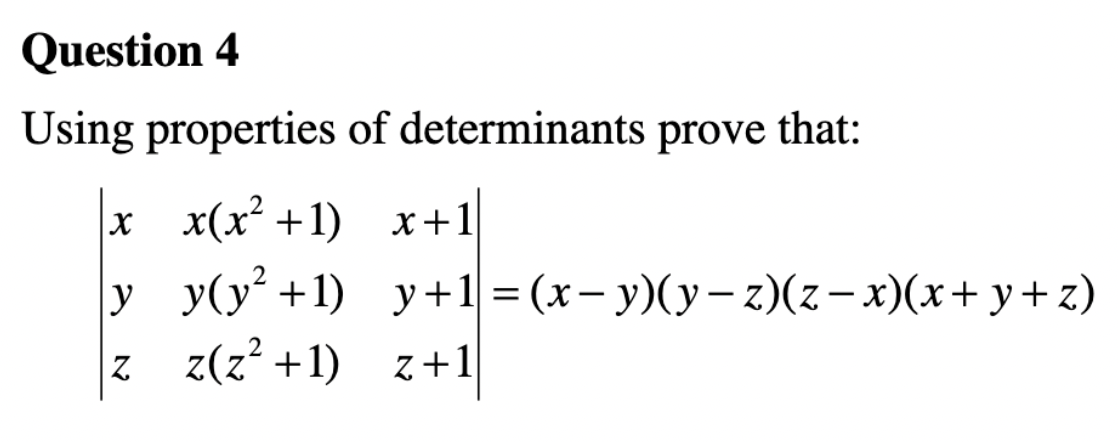
\includegraphics[width=9cm]{question.png}
   \textbf{Solution:}Given Matrix, let M
\end{figure}
M=
\begin{vmatrix}
x &x(x^2+1) &x+1\\
y &y(y^2+1) &y+1\\
z &z(z^2+1) &z+1
\end{vmatrix}
\\
\\Using Split property of determinant at column 3 we get 
\\
\\M=
\begin{vmatrix}
x &x(x^2+1) &x\\
y &y(y^2+1) &y\\
z &z(z^2+1) &z
\end{vmatrix}
+
\begin{vmatrix}
x &x(x^2+1) &1\\
y &y(y^2+1) &1\\
z &z(z^2+1) &1
\end{vmatrix}
\\
\\ As \nth{1} and \nth{3} coloumns of \nth{1} determinant are same it's value becomes zero then
\\
\\M=
\begin{vmatrix}
x &x^3+x &1\\
y &y^3+y &1\\
z &z^3+z &1
\end{vmatrix}
\\
\\Using Split property of determinant at column 2 we get 
\\
\\M=
\begin{vmatrix}
x &x^3 &1\\
y &y^3 &1\\
z &z^3 &1
\end{vmatrix}
+
\begin{vmatrix}
x &x &1\\
y &y &1\\
z &z &1
\end{vmatrix}
\\
\\ Similarly as \nth{1} and \nth{2} coloumns of \nth{2} determinant are same it's value becomes zero then
\\
\\M=
\begin{vmatrix}
x &x^3 &1\\
y &y^3 &1\\
z &z^3 &1
\end{vmatrix}
\\
\\Using row transformation properties i.2 changing row1 to (row1-row2) and row2 to (row2-row3) we get
\\
\\M=
\begin{vmatrix}
x-y &x^3-y^3 &0\\
y-z &y^3-z^3 &0\\
z &z^3 &1
\end{vmatrix}
\\
\\Evaluating the determinant of matrix at (3,3) position we get value of determinant as 
\\
\begin{sol}
\\	&= (y^3-z^3)(x-y)-(y-z)(x^3-y^3) \\
\\
	&=(y-z)(y^2+z^2+y.z)(x-y)-(y-z)(x^2+y^2+x.y) \\
\\
	&=(y-z)(x-y)[y^2+z^2+y.z-x^2-y^2-x.y]\\
\\
	&=(y-z)(x-y)[(z-x)(z+x)+y(z-x)]\\
\\
	&=(y-z)(x-y)(z-x)[z+x+y]
\end{sol}
\\By rearranging the terms we get the value of determinant as
\\&=(x-y)(y-z)(z-x)(x+y+z)
\\=R.H.S
\\Hence proved!
\\THe following is a result of c code with takes inputs for x,y,z and checks whether both LHS and RHS are equal
\\
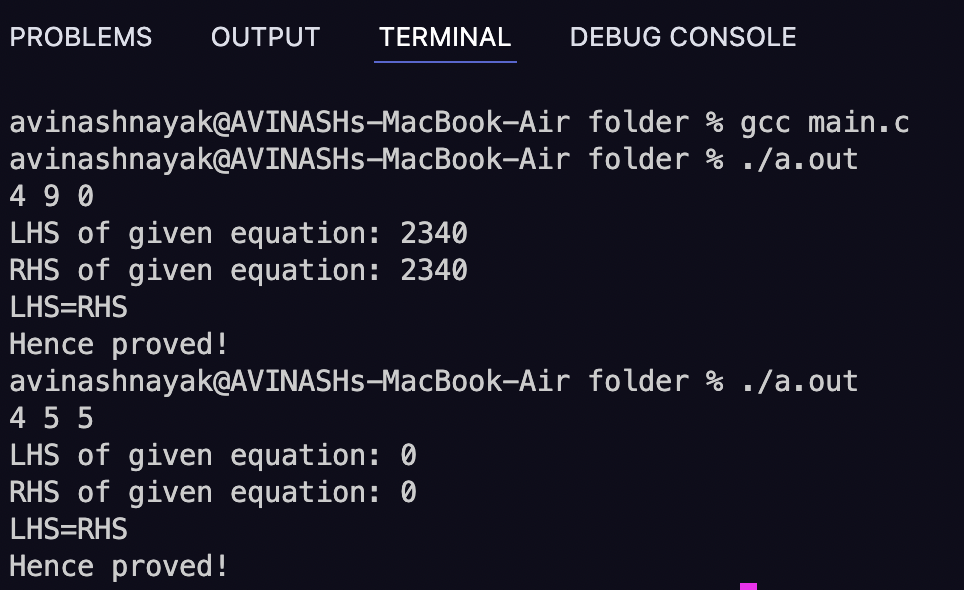
\includegraphics[width=9cm]{solution.png}

\end{document}